\section{Introduction}
In many applications, image denoising is used to produce good estimates of the original image from noisy observations.   The restored image should contain less noise than the observations while still keep sharp transitions (i.e. edges). \\


Wavelet transform, due to its excellent localization property, has rapidly become an indispensable signal and image processing tool for a variety of applications, including 
compression and denoising \cite{21,22,23}.   Wavelet denoising attempts to remove the noise present in the signal while preserving the signal characteristics, regardless of its 
frequency content.   It involves three steps:a linear forward wavelet transform, nonlinear  thresholding step and a linear inverse wavelet transform.\\

Wavelet thresholding (first proposed by Donoho \cite{21,22,23}) is a signal estimation technique that exploits the capabilities of wavelet transform for signal denoising.   It removes noise  by killing coefficients that are insignificant relative to some threshold, and turns out to be simple and effective, depends heavily on the choice of a thresholding parameter and the choice of this threshold determines, to a great extent the efficiency of denoising. Researchers have developed various techniques for choosing denoising parameters and so far there is no "best" universal threshold determination technique. \\

In my method i decompose the image by MST used in the transformation then apply BayesShrink soft thresolding to remove the insignificant coefficient the The aim of this project was to study various thresholding techniques such as  SureShrink \cite{21}, VisuShrink \cite{23} and BayesShrink \cite{22} and determine the best one for image 
denoising.

\section{Hard and soft thresholding}

Hard and soft thresholding with threshold ¸ are defined as follows: \\
The hard thresholding operator is defined as:
\begin{equation}
    \begin{split}
  D(U,T)=
\begin{cases}
 T& \text{ if } U>T \\
 0 &\text{ if } otherwise  
\end{cases}
    \end{split}
\end{equation}
The soft thresholding operator on the other hand is defined as:
\begin{equation}
D(U,T)=sgn\left(U \right)\max \left(0,\mid U \mid-\lambda  \right)
\end{equation}

\begin{figure}[h!]
  \centering
  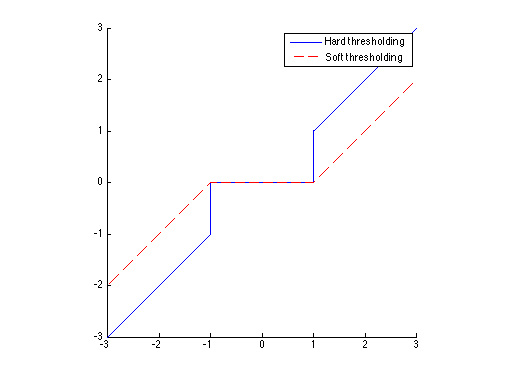
\includegraphics[width=.8\textwidth]{4a.png}
  \caption{soft and hard thresholding} \label{tsr}
\end{figure}

Hard threshold is a “keep orkill” procedure and is moreintuitively appealing. The transfer function of the same is shown in Fig \ref{tsr}. The alternative, soft thresholding  
(whose transfer function is also shown in Fig \ref{tsr}), shrinks coefficients above the threshold in absolute value. While at first sight hard thresholding may seem to be natural, the continuity of soft thresholding has some advantages. It makes algorithms  mathematically more tractable \cite{23}. Moreover, hard thresholding does not even work with some algorithms such as the GCV procedure . Sometimes, pure noise 
coefficients may pass the hard threshold and appear as annoying ’blips’ in the output. Soft thesholding shrinks these false structures. 

\section{Image denoising using thresholding}
As one may observe, threshold selection isan important question when denoising. A small threshold may yield a result close to the input, but the result may still be noisy.   A 
large threshold on the other hand, producesa signal with a large number of zero coefficients.   This leads to a smooth signal.Paying too much attention to smoothness, however, destroys details and in image processing may cause blur and artifacts. \hfill \break
The problem boils down to finding an optimal threshold such that the mean squared error  between the signal and its estimate is minimized. The wavelet decomposition of an 
image is done as follows: In the first level of decomposition, the image is split into 4 subbands, namely the HH, HL, LH and LL subbands. The HH subband gives the diagonal details of the image; the HL subband gives the horizontal features while the LH subband represents the vertical structures. The LL subband is the low resolution residual consisting of low frequency components and it is this subband which is further  split at higher levels of decomposition.  The different methods for denoising investigate differ only in the selection of the threshold. \hfill \break
I use the above perception of denoising for every MST i used.
So the basic procedure is 
\begin{itemize}
\item Calculate the MST coefficient of the image
\item Threshold the coefficient
\item Inverse transform the coefficient to get the denoised image.
\end{itemize}

\subsection{BayesShrink}
BayesShrink is an adaptive data-driven threshold for image denoising via wavelet soft-thresholding.The threshold is driven in a Bayesian framework, and we assume 
generalized Gaussian distribution (GGD) for the wavelet coefficients in each detail subband and try to find the threshold T which minimizes the Bayesian Risk.It is  found that BayesShrink performs better than SureShrink in terms of MSE. The reconstruction using BayesShrink is  smoother and more visually appealing than one obtained using SureShrink. 
\hfill \break

The BayesShrink threshold is given by :
\begin{equation}\label{bayest}
\hat{T}\left(\hat{{\sigma }_{I}} \right)=\frac{\hat{{\sigma }_{n}}}{\hat{{\sigma }_{I}}}
\end{equation}

where \({\sigma}_{n}\) and \({\sigma}_{I}\) are noise and signal standard deviations respectively.To estimate the noise variance\({\sigma}_{n}^{2}\) from the subband details, the median estimator is used on the 1-D subband coefficients:

\begin{equation}
\hat{{\sigma }_{n}}=median\left(\mid Details  \mid  \right)/0.6745
\end{equation}
the observed signal S is considered to be \( S=I+n\) and signal (I) and noise (n)are assumed to be independent.Therefore, 
\begin{equation}
\sigma _{S}^{2}=\sigma_{I}^{2}+\sigma_{n}^{2}
\end{equation}
where \(\sigma_{S}^{2} \)is the variance of the observed signal. So \(\sigma_{I}^{2}\)is estimated by:
\begin{equation}
\hat{\sigma_{I}}=\sqrt{\max\left(\left(\hat{{\sigma}_{S}^{2}}-\hat{\sigma _{n}^{2}} \right),0 \right)}
\end{equation}








